\section{Cadre idéal}

Nous avons effectuer différents tests durant le projet. En utilisant les vidéos fournis sur le site du MIT. Notre logiciel arrive à obtenir des 
résultats très correct. En effet, par exemple comme on peut le voir sur cette capture d'écran. Après notre magnification réalisé, on retrouve
une fréquence cardiaque d'environ 53 battements par minute (BPM), l'article du MIT lui trouve une fréquence de 54 BPM.  

\begin{figure}[h!]
	\centering
	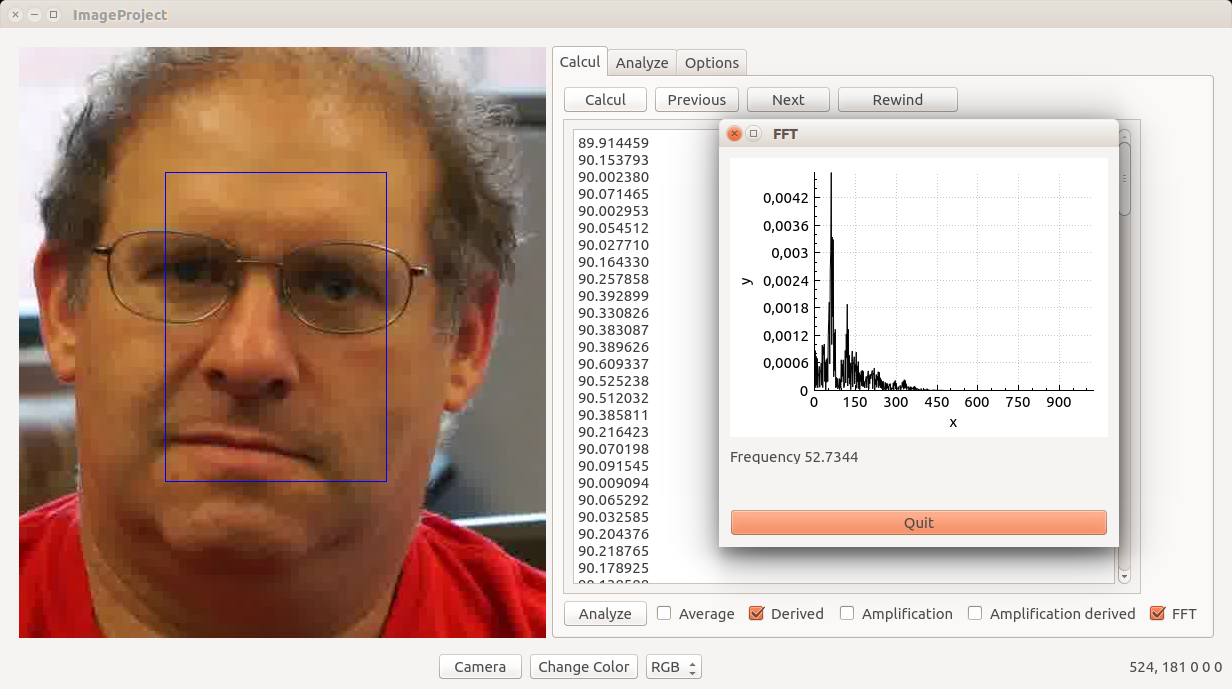
\includegraphics[width=0.9\textwidth]{data/cas-ideal.png}
	\caption{Vidéo source du MIT analysé avec notre logiciel.}
\end{figure}


\section{Webcam}

Avec une webcam, nos résultats sont moins précis, mais sont assez correct pour être utiliser. 

capture webcam here

\section{Android}

Notre plus gros problème a bien entendue était lors de nos tests sur Android, la stabilité de la vidéo et le nombre de frames capturés.
Actuellement notre application est capable de capturer des frames et appliqué notre algorithme mais nos résultats restent éronnés.
